\section{长度测量的一些特殊方法}\label{sec:1-2}

长方形的长和宽、正方体的边长、圆柱体的高等直线长度,都可以用刻度尺直接测量。
铁路、公路、跑道等往往是弯曲的,曲线的长度怎么测量呢?
圆锥体的高虽然是直线,但是用刻度尺却很难测准。这又怎么办呢?
用有毫米刻度的尺无法直接测出一张纸的厚度,而我们要知道这个厚度,又没有更精密的尺,该怎么测量呢?

对于这些不能直接用刻度尺测出的长度,要根据具体情况想些特殊的方法。


\begin{figure}[htbp]
  \centering
  \begin{minipage}{9cm}
  \centering
  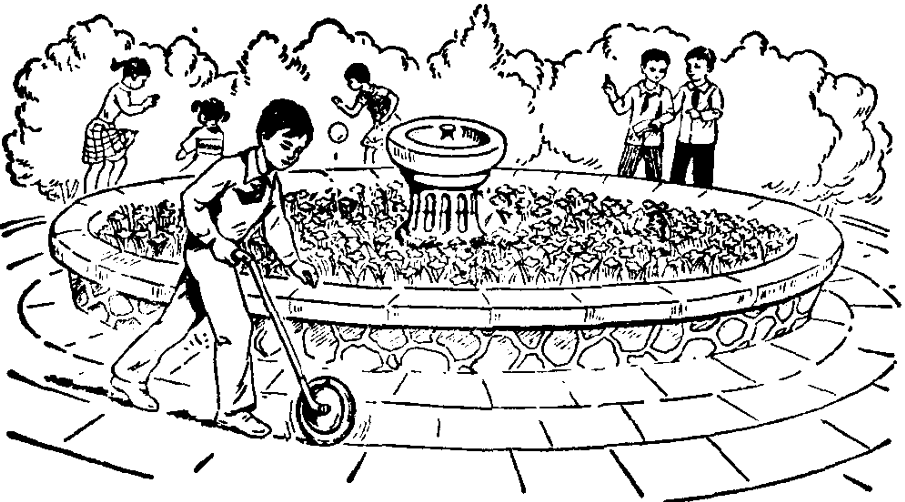
\includegraphics[width=9cm]{../pic/czwl1-ch1-7}
  \caption{}\label{fig:1-7}
  \end{minipage}
  \qquad
  \begin{minipage}{4cm}
  \centering
  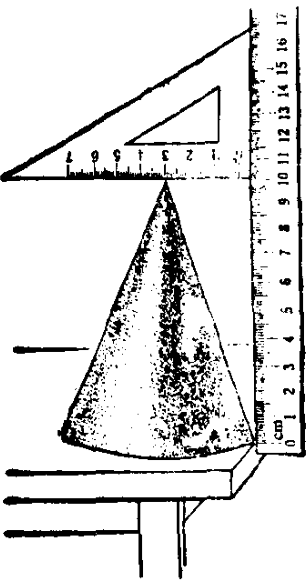
\includegraphics[width=3.5cm]{../pic/czwl1-ch1-8}
  \caption{}\label{fig:1-8}
  \end{minipage}
\end{figure}

曲线的长度可以用一个轮子沿着曲线滚动,测出轮子的周长,记下滚过的圈数,用轮子的周长乘以圈数,
就可以得到曲线的长度(图 \ref{fig:1-7})。火车、汽车上记录行驶路程的里程表,就是根据这个道理制做的。
比较短的曲线可以利用一条弹性不大的柔软棉线来测量。
先把棉线放在曲线上,让它跟曲线完全重合,在棉线上标出曲线的起点和终点,然后把棉线放直,
量出棉线上两点间的距离,就得到了曲线的长度。


圆锥体的高可以照图 \ref{fig:1-8} 那样,用直角三角板和刻度尺配合进行测量。

用有毫米刻度的尺测不出一张纸的厚度,也测不出两张纸的厚度,但是能测出 100 张纸的厚度。
把测出的厚度除以总张数,就得到一张纸的厚度。

\lianxi

(1) 用有毫米刻度的尺,近似地量出练习本里一张纸的厚度。

(2) 用刻度尺和三角板测量乒乓球的直径(图 \ref{fig:1-9})。


\begin{figure}[htbp]
  \centering
  \begin{minipage}{6cm}
  \centering
  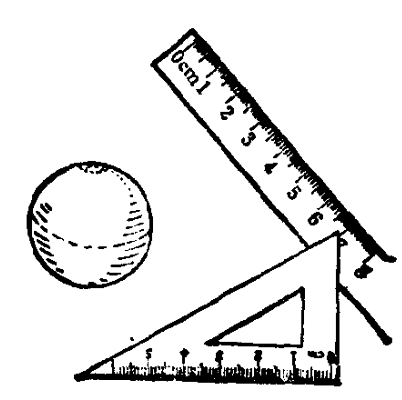
\includegraphics[width=6cm]{../pic/czwl1-ch1-9}
  \caption{}\label{fig:1-9}
  \end{minipage}
  \qquad
  \begin{minipage}{4cm}
  \centering
  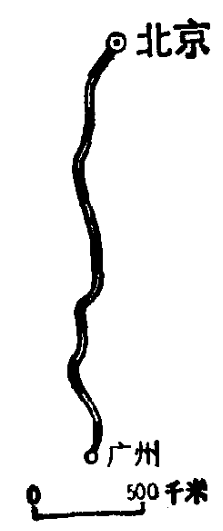
\includegraphics[width=2.5cm]{../pic/czwl1-ch1-10}
  \caption{}\label{fig:1-10}
  \end{minipage}
\end{figure}

(3) 测量图 \ref{fig:1-10} 中京广铁路线的近似长度(用千米作单位)。

(4) 先用刻度尺量出你步行时两脚间的距离,即一步的长度,然后测出篮球场的长和宽各是多少步,
再算出篮球场的长度和宽度。


\nonumsection{小实验: 测量细金属丝的直径}

找一支圆铅笔,一把有毫米刻度的尺,一段长 50 厘米左右的细金属丝。
想办法用刻度尺量出细金属丝的直径。


